\documentclass[a4paper,man,natbib]{apa6}
%\usepackage[square]{natbib}
\usepackage{microtype}
\usepackage{mathtools} % needed
\usepackage{hyperref}
\usepackage{tabularx}
\newcolumntype{Y}{>{\raggedright\arraybackslash}X}

\usepackage[normalem]{ulem}
\hypersetup{hidelinks=True}
\usepackage{lingex} % some linguistic-style example numbering

\newcommand*{\smex}[1]{\textit{#1}} % 'small example'
\newcommand*{\spex}[1]{``{#1}''} % 'spoken example'
\newcommand*{\term}[1]{\emph{#1}} % introducing a new term
\newcommand*{\citegen}[1]{\citeauthor{#1}'s~(\citeyear{#1})}
\newcommand*{\SE}{\mathit{SE}} % fix funny "SE" spacing
\newcommand{\resultsLog}[3]{$\beta = #1$, $\textnormal{SE} = #2$, $p #3$}
\newcommand{\resultsLM}[3]{$\beta = #1$, $\textnormal{SE} = #2$, $t #3$}

\title{<Martin's pithy title about gesture and speech>.}
\author{JK, MC, HR}
\affiliation{Psychology, PPLS, University of Edinburgh}
\ifapamodeman{\note{\begin{flushleft}%
Josiah King\\
Philosophy, Psychology and Language Sciences\\
University of Edinburgh\\
7~George Square\\
Edinburgh EH8~9JZ, UK\\[1ex]
\url{J.P.J.King@sms.ed.ac.uk}
\end{flushleft}}}

\shorttitle{e5 - gesture production}

\abstract{                   
When a task becomes more conceptually demanding, speakers tend to produce more gestures.  This might be because gestures help the speaker package more complex information into appropriate units for speech, or because some of the communicative load is being traded off from speech to gesture.  The present study is a dialogue study designed to tease apart these views.

Previous research has found evidence for both views.  Speech and gesture have been found to specify referents in parallel, but a general increase in gesture duration over a trial has been found when referents are less describable.

Studies such as these have tended to look at the relationship between gesture and speech where there is no addressee, or where the addressee is not explicitly contributing to a dialogue.  Moreover, gesture has tended to be measured as the number of discrete gestures per word or trial.  Because gestures and vocalisations can vary in durations, these metrics fail to capture the relative contributions of each. In the present study we use naturalistically-occurring dialogues, and measure the relative durations of gestures and speech directly, in order to establish whether they co-vary (as would be predicted by the packaging account) or correlate inversely (as would be predicted by a trade-off).

Twenty-two pairs of participants took part in a shape-matching game, in which a director described two target shapes, and a matcher attempted to identify the correct referents among an array of competitors.  Roles alternated on each trial, and the shapes were either easy or difficult to verbally encode.  Directors saw two shapes (one easy, one difficult) for two seconds. They then had 10 seconds to describe these shapes to their partner.  Points were scored for each shape which the matcher correctly identified in an array of six shapes.

In line with an information packaging account, speech duration and gesture duration increased in parallel for easy-to-name objects \resultsLM{0.57}{0.06}{>2}.  Importantly, when participants were referring to objects which were more difficult to verbally encode, gesture duration increased at a higher rate than speech duration \resultsLM{0.27}{0.06}{>2}.

This suggests that, when naming difficult objects, gesture does more than simply help the speaker to package verbal information.  Instead, gesture serves an additional communicative purpose, adding to, but not trading off against, the verbal descriptions which are uttered.
}

\begin{document}
\maketitle


\noindent
During conversation, speakers often move their hands and arms in meaningfuls ways which co-express the content of their speech \citep{McNeill1992}:%JK is this a bad opener, given that we're asking how much of gesture "co-expresses" speech and how much it takes over?
These movements might add emphasis to speech; indicate location; or depict properties of objects, movements, actions or space.
Research suggests that when a task becomes more conceptually demanding, speakers tend to produce more gestures.
This might be because gestures have benefits for speech, either in aiding lexical access \citep{Rauscher1996, Krauss2000} or in helping to package more complex information into appropriate units for speech\citep{Kita2000}.
Alternatively, gesture production might increase with conceptual demand because some of the communicative load is being traded off from speech to gesture \citep{Melinger2004, Bangerter2004, DeRuiter2006}.

In contrast to common methods of measuring the number of discrete gestures per word, experimental trial or some other construct, the present study measures the relative durations of gestures and speech directly, in order to establish whether they co-vary (as would be predicted by a gesturing-to-benefit-speech account) or correlate inversely (as would be predicted by a trade-off).
With few studies having investigated the speech-gesture relationship in a dialogical setting where two people are making explicit contributions, we use naturalistically-occurring dialogues in which participants jointly engage in producing referring expressions.

Although gesturing has traditionally been considered to be intended to directly communicate meaning to an addressee, recent research has suggested that it may in part be motivated by the cognitive benefits it has for the speaker.
Advantages of gesturing have been found in many areas: In speech production and planning processes \citep{Rauscher1996, Krauss1999, Rose2001, Morsella2004, Kita2000}; spatial working memory \citep{Wesp2001, Morsella2004}; conceptual planning \citep{Melinger2007}; and even doing mental arithmetic \citep{Goldin-Meadow2001}

Explanations of the mechanism by which gesturing may benefit production of speech have been varied. 
One suggestion holds that gesturing increases activation on relevant items in the mental lexicon, thus facilitating access \citep{Krauss2000}. Another \citep{Hadar1997} suggests that gesturing prevents visuo-spatial imagery from decaying, providing speech production processes with higher quality information. In a similar vein, the Information Packaging Hypothesis \citep{Kita2000, Kita2003} claims that gesturing helps speakers to package complex information into appropriate units for speech. 

Common to all these accounts is the claim that as conceptual load increases, speech and gesture increase in parallel.
A \citeyear{So2009} study from \citeauthor{So2009} found evidence which patterned with this claim. 
Participants were asked to describe scenes from videotaped vignettes (e.g., a man giving woman a basket) and their use of both speech and gesture to indicate characters in the scene was measured.
\citeauthor{So2009} found that speakers more often used a gesture to identify a referent if it was also specified in speech. 
\citeauthor{So2009} viewed their results as evidence in support of an account of speech and gesture going `hand-in-hand' --- i.e. the two modalities co-varying.

However, where \citeauthor{So2009}'s participants did not use gesture to compensate for underspecifications in their spoken descriptions, other studies have found contrasting results.
In \citet{Melinger2004}, participants were asked to communicate information to an interlocutor about the spatial arrangements of connected dots of different colours. 
As it was possible to determine the minimal content necessary for each of the stimuli \citeauthor{Melinger2004} were able to measure whether omissions in speech were accompanied by compensatory gestures. 
\citeauthor{Melinger2004} found that people who gestured produced more --- and different --- omissions in speech than people who did not. 

\citeauthor{Melinger2004}'s results pattern with other studies \citep{Bangerter2004, DeRuiter2006, VanderSluis2007} in which the informational content of speech is found to inversely correlate with the amount or precision of gestures. 
Observations such as these provide evidence for a trade-off relationship between speech and gesture --- in some cases at least, gesturing appears to assume some of the communicative load from speaking.
The trade-off account holds that speakers distribute communicative load across speech and gesture such that that when speaking becomes more difficult, gesturing will increase (and vice versa). 
This view directly contrasts with the co-varying account, suggesting that as it becomes harder to verbally encode meaning, rates of speech will decrease while rates of gesture will increase. 



\hrule
\vspace{5em}
JK up to here
\vspace{5em}
\hrule


\subsubsection{why?}
There are various possible reasons for the varied accounts of how speech and gesture interact. 

One explanation is that the speech-gesture relationship might depend on the type of gesture in question.
Several studies have found evidence suggesting that some types of gestures are intended to communicate whilst others are not.
\citet{Alibali2001} found that speakers' who could see their addressee used more \term{representational} gestures, but not \term{beat} gestures. 
Similarly, \citet{DeRuiter2012} found mutual visibility to influence pointing and \term{obligatory iconic} gestures more (gestures containing information not represented in speech but required for disambiguation), but not \term{non-obligatory iconic} gestures (gestures which are not essential to the understanding of co-occurring speech).

Much of this also depends on the setup of the experiment and the stimuli used. 
Manipulating the describability of pictures, \citet{DeRuiter1998} found no change in gesture rate.
However, as \citet{Morsella2004} point out, what \citeauthor{DeRuiter1998} varied was complexity, and not describability. 
In a study designed to tease apart these two concepts, \citet{Morsella2004} concluded that while visual complexity did not affect gesture rates, verbal codability did, with harder-to-name pictures eliciting higher rates of gesturing.
To make matters worse, in a \citeyear{DeRuiter2012} study, \citeauthor{DeRuiter2012} found no effect of verbal codability on speakers' rates of gesturing. 

It might be that differences such as these are due to something as simple as the physical orientation of participants in relation to each other and the stimuli. 
In \citet{DeRuiter2012}, participants appeared to sit facing at an angle 45 degrees between each other and a jointly visible set of stimuli. 
A setup such as this is likely to favour pointing at the referent at least as much as iconically representing it in space.
With pointing being of comparatively low effort, 









Additionally, \citet{Mol2011} found that over computer-mediated conversation, more gestures were produced when participants knew they were visible to the addressee than when the addressee was visible to them, suggesting that these gestures were produced to be seen. 
\citeauthor{Mol2011}'s finding reflects that of \citet{Bavelas2002}, in which participants described stimuli to a supposed future addressee who would receive either audio or audiovisual recordings. \citeauthor{Bavelas2002}'s results showed participants gesturing more when they believed their descriptions would be seen by the future addressee.
It is not just the visible presence of an addressee which influences a speaker's gesturing: Several studies suggest that speakers tailor their use of gesture to specific contexts and addressees:
As well as mutual visibility \citep{Alibali2001, Cohen1973, Hoetjes2015}, an increase in the quantity or precision of speakers' gestures has been associated with less common ground \citep{Gerwing2004, Holler2007}, and information which is novel for the addressee \citep{Jacobs2007}.\\



\subsubsection{problems - G-rate dialogue}
%identify two problems with previous studies. gesture rate and monologue.
%gesture rate measures.
One reason for the mixed results in studies surrounding how speech and gesture interact may be the differences in how the relationship between the two is measured:
Tending towards \term{rate} measures (i.e. gesture as a function of speech), studies have differed in their choice of measures for both modalities.
Much research has involved measuring the number of discrete gestures produced when speaking (e.g. \citet{Hostetter2007, Gerwing2011, DeRuiter2012, Hoetjes2015}).
However, coding a speaker's arm movements into distinct gestures is not straightforward.
Unlike speech --- where distinct phonemes and words offer comparatively clear means of measuring utterance length and duration --- multiple pieces of information (and multiple types of gesture) may be produced in the time between the raising and lowering of hands.
In the literature, defining individual gestures has varied with the thing being described, from ``illustrating a feature of the target (for instance its shape).'' when describing tangram figures \citep{DeRuiter2012} to change in any one of ``shape and placement of the hand, trajectory of the motion'' when identifying referents in a narrative \citep{So2009}.
Furthering to this confusion, rates of discrete gestures have been calculated per minute \citep{Mol2011}; per 100 words \citep{Masson-Carro2015, Hostetter2007, Gerwing2011, Hoetjes2015}; per \term{feature description} 
tep{DeRuiter2012} or per \term{semantic attributes} \citep{Hoetjes2015}.\\




%our measure
For representational/iconic gesturing, we propose that a duration-based account offers a simpler (but underused) measure.
This measure involves simply comparing the durations for which a speaker conveys (or attempts to convey) information via different channels. 
Gesturing is often considered to be split into three main phases: Preparation; Stroke or Hold; and Retraction \citep{McNeill1992}.
Excluding the prepatory and retraction phases, comparing the duration for which a speakers hands are in the air with the duration for which they are speaking offers a more objective measure of how 
information is distributed in multimodal communication.
%Because gestures contain `disfluent' movements (e.g. hand hanging in mid-air), taking the duration of gesturing as a function utterance duration (which includes disfluencies) allows for a direct comparison of the time a speaker spends describing in either modality.



%dialogue
Much of the evidence above suggests that the addressee plays an important role in a speaker's use of speech and gesture.
Additionally, gesturing is often useful for the addressee (for an overview, see \citet{Hostetter2011}). 
Despite this, there has been little research into how speech and gesture interact in a truly dialogical setting.
To date, much of the research into gestures has involved studies in which a single speakers' gestures are evaluated under various conditions.
Experimental paradigms have tended towards those in which participants produce speech and gesture either to an imagined future addressee (e.g. \citet{Wesp2001, Morsella2004}) or to an addressee who is present but in a comparatively passive role (e.g. a "matcher" to a "director", as in \citet{Bangerter2004, Holler2007, DeRuiter2012, Hoetjes2015}).
These sorts of designs fail to capture the dynamic process of conversation - that is, the fact that dialogue is a joint activity \citep{Clark1996}.\\

A study by \citeauthor{Bavelas2008} showed independent effects of visibility and dialogue on gesturing:
Speakers produced more gestures when speaking to an occluded but dialogically involved listener than when speaking to a tape recorder. 
Furthermore, recent research suggests that speakers will mimic their interlocutors gestures \citep{Kimbara2008, Holler2011}. %JK these studies didn't look at speech so much. 
%JK i need to talk about convergence - on sp or g? 



\subsubsection{presently...}
%present study










\section{Experiment}

\subsection{Setup}
Pairs of participants engaged in a collaborative matching game, in which they were tasked with matching two target shapes seen by one particpant from a set of six shapes seen by the other participant. 
Participants took turns in the roles of \term{director} and \term{matcher}.
Target shapes varied in verbal codability: they were either easy- or hard-to-name.
We also manipulated participants' familiarity with the target shapes in both roles (director and matcher).


\subsection{Materials}
Pairs of shapes in critical trials were selected from a set of 20 critical shapes (10 easy-to-name, 10 hard-to-name).
Each of the 10 easy-to-name shapes was altered (sections of the shape were rotated and/or flipped) to create the 10 hard-to-name variants. %JK see fig!
For filler trials, shapes were selected from a further set of 40 shapes (20 easy-to-name shapes and 20 hard-to-name variants). 

A set of 20 \term{distractor} shapes (10 easy-, 10 hard-to-name) were visually and descriptively similar to the 20 critical target shapes. %JK REWORD, give example
These shapes were never described, only being presented as part of the matchers' arrays, with the aim of encouraging specificity in future descriptions.

In critical trials, the two shapes seen by the director differed in codability.
In filler trials, target shapes were both the same codability (both easy-to-name or both hard-to-name).

Matchers' arrays were composed of six shapes.
Along with the two target shapes for that trial, this was comprised of two randomly selected filler shapes and two randomly selected distractor shapes. 
Codability of the shapes in the array matched that of the target shapes (i.e. for critical trials, half were easy-to-name, half were hard-to-name).
Positions of shapes were randomly selected for both the director (Left vs.\@ Right) and for the matcher (in a 2x3 grid).


\subsection{Experimental blocks}

The experiment consisted of two blocks, each containing 40 trials (20 critical and 20 fillers). 
In each block, every critical shape was seen twice.

In the first block, critical trials were sampled without replacement from a list of 20 trials, with the constraint that target shapes were never repeated in consecutive critical trials.
Whilst the majority of the shapes were described once by each participant, the probability that a given shape was described twice by the same participant was 25\%\footnote{Whilst the intention was to make it so that each participant described each critical shape once, a typing error in the experiment script resulted in these distributions}. 

For the 20 filler trials, two target shapes of the same codability were randomly selected from the set of filler shapes.

In the second block, pairs of consecutive critical trials alternative with pairs of filler trials. 
For the consecutive critical trials, the difficult-to-name shape was repeated.
This meant that for critical trials where participant B was the director, they were tasked with describing the difficult shape which had just been described to them in the previous trial by participant A.
Filler trials remained the same as in block 1. 


\subsection{Procedure}
Participants sat facing each other on chairs (without any arms), with an unobstructed view of each other.
Each participant had a monitor and a mouse on a table to their left, positioned such that they could not see what was on their partner's monitor.
The setup was designed to encourage face-to-face dialogue, and to discourage participants from leaving their hand resting on the mouse whilst speaking (the position being uncomfortable for a right-handed mouse user), thus leaving both arms free to gesture.
Audio and video was recorded by two cameras positioned to the right of each participant, facing their partner.

Taking turns in the roles of director and matcher, participants were tasked with successfully matching what was seen on the director's monitor from a set of possibilities on the matcher's monitor.

As a pair, participants were awarded points for successful matching.
As an incentive, the highest scoring pair received £40, and participants were informed of this beforehand.

A high-score table was shown prior to the experiment, with participants adding their score to the table after they had played.
To encourage face-to-face dialogue, participants were only allowed to communicate within a restricted time-window of 10 seconds during which no images were present on either screen. 
Participants were told that during this period, they were "both allowed to talk, gesture, ask questions, and so on". 
Thus gesturing was permitted but not explicitly encouraged.
The end of this window was signified by the sound of a bell (see Figure \ref{fig:trial}).

Feedback was given at the end of each trial (The number of correctly matched shapes was signified by an equivalent number of bell rings, with zero correct resulting in a buzzer), and the participants' cumulative score was displayed.

\begin{figure}
  \centering
	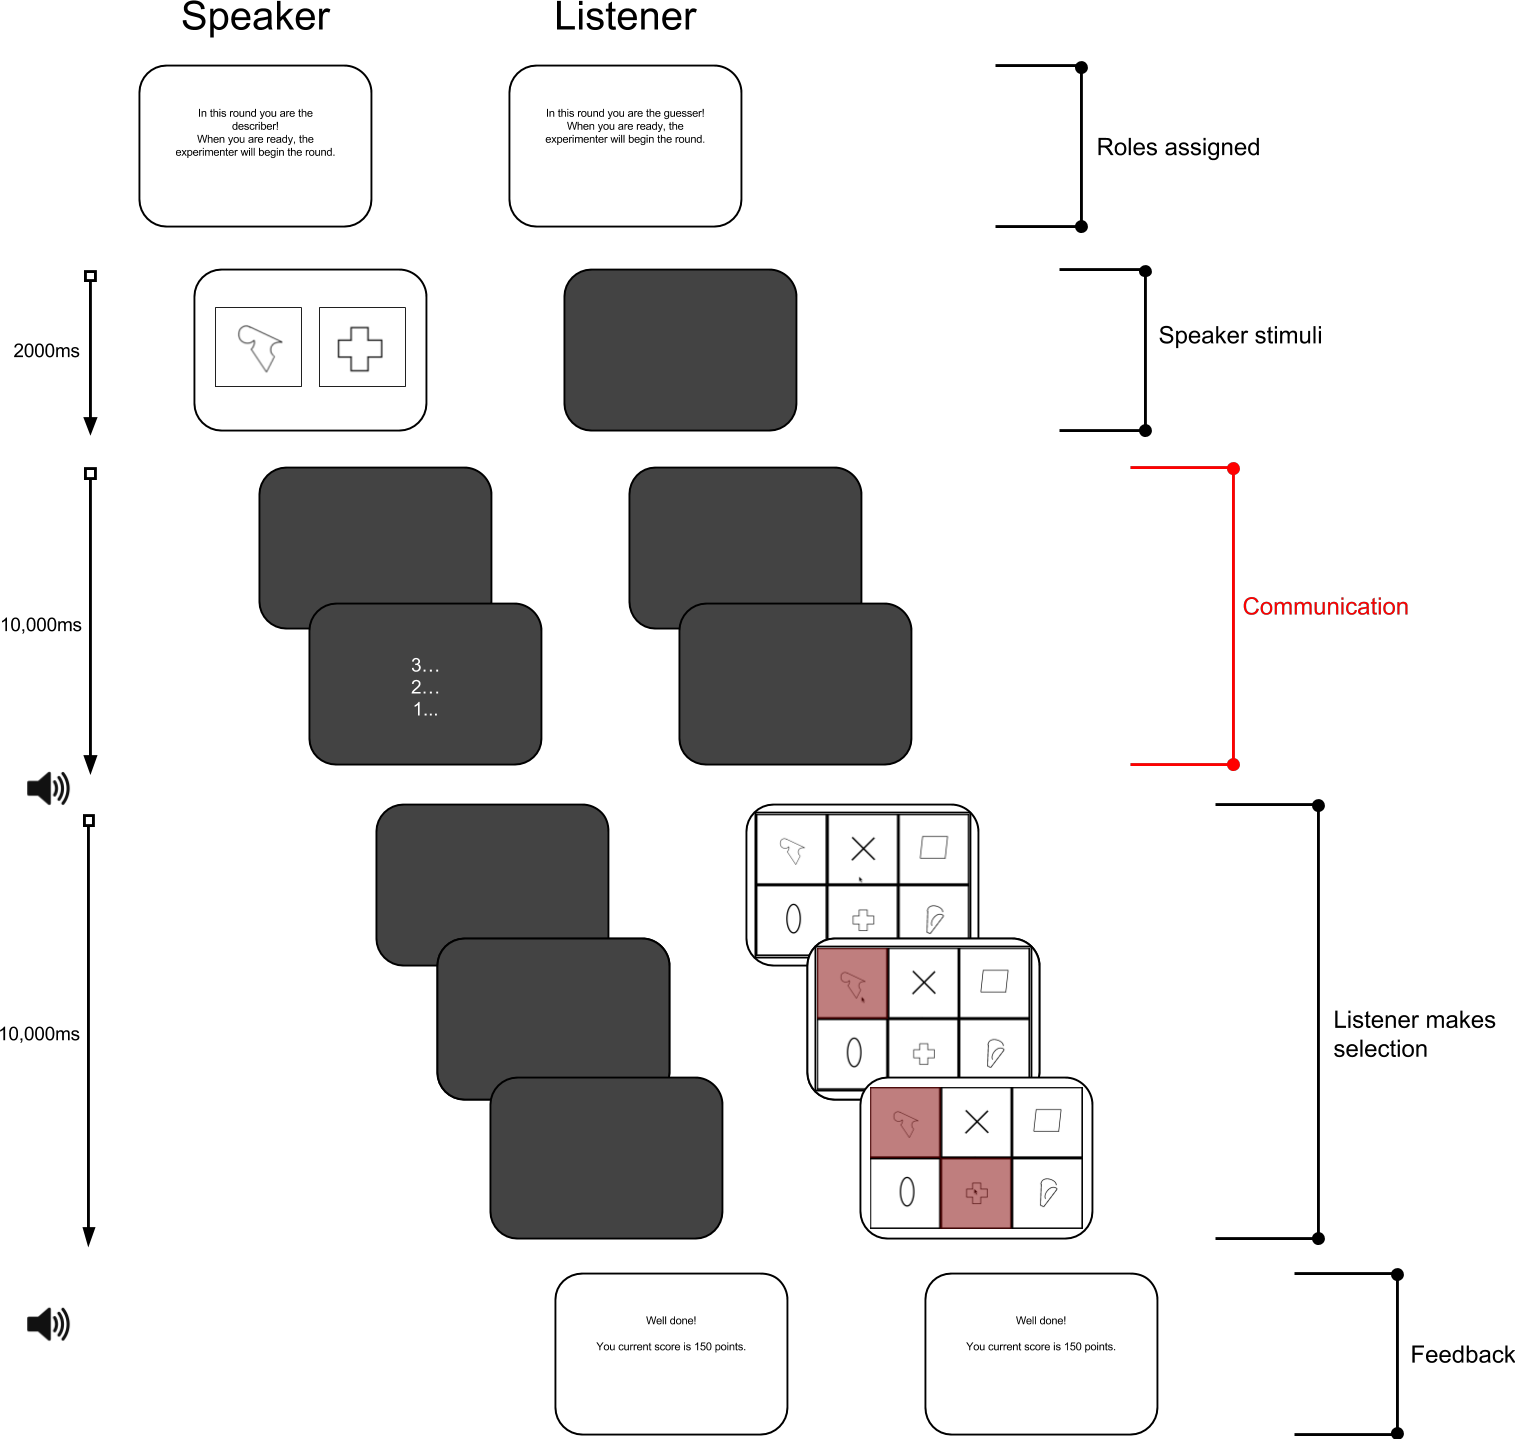
\includegraphics[width=\linewidth]{trial.png}
  \caption{Procedure of a given trial.}
  \label{fig:trial}
\end{figure}

\section{Coding}
Audiovisual data for each pair of participants was coded using a three stage process:
Audio-only and Video-only stages were used to code for speech and gesture respectively, with the third stage (both Audio and Video) used to confirm the variables resulting from the previous stages.
As each trial consisted of describing two shapes, special care was taken in the third stage to ensure that utterances and gestures were assigned to the correct referents\footnote{There was potential for descriptions in both modalities to merge into one another}.
%JK reword footnote?


\subsection{Speech Coding}
Utterance duration, utterance length and disfluencies were coded in the Audio-only stage.
Only the first mention of each shape was used. 
Utterance duration (ms) was coded from the onset of the noun-phrase up until either a) speech-offset, or b) a valid interruption from the listener in either modality.
Listeners' use of the collateral channel (for instance: "yep","mmhm",[nods head]) were not considered valid interruptions.
Utterance length (number of words) was coded analogously, with disfluencies within the utterance period being identified and excluded from this measure.

Disfluencies were coded as falling into one of six categories: Filled pauses; Insertions; Substitutions; Articulation Errors; Deletions; Repetitions. 
(ref Shriiberg).
Any speech prior to the onset of the noun-phrase was coded as either fluent or disfluent.

Conceptual pacts were coded during the third (both Audio and Video) stage. 
%JK HOW DO WE CLASSIFY CONCEPTUAL PACTS. definite descriptions "THE","again","another". 



\subsection{Gesture Coding}
Gestures were identified in the Video-only stage of the coding process.
Any movement from the fingers up to the shoulder were considered. 
Only gestures which partially overlapped an identified utterance period were included, and were assigned to the utterance which they primarily overlapped. 
This pairing was then confirmed in the third stage of the coding process. 
In any cases of a gesture being ambiguous as to which utterance it accompanied (i.e. adaptor gestures which overlap both utterance periods), the gesture was assigned to both referents.

Gestures were categorised in to five types: Iconics; Beats; Points; Adaptors; and Others. 
Any gesture which was considered to be an attempt to represent any feature of the target shape was coded as an Iconic gesture.
Beat gestures were identified as any movements which rhythmically matched prosody in speech but which \emph{did not} represent any feature of the target shape.
Point gestures were extensions of the index finger used to refer deictically to either present objects or people, or to previous parts of the discourse.
%JK give examples ?
Other movements were categorised as either adaptor gestures (scratching, stroking, manipulating clothing, etc.), or other miscellaneous gesticulations.

Individual gestures were identified by onset of movement, and continued either until the start of the retraction phase, or until transformation into a) a different category of gesture or b) iconic gesturing referring to a different shape\footnote{Because each trial involved a participant describing two shapes...}. 

The third stage of the coding process (audio and video) was used to confirm the coding of the first and second stages, specifically gesture categorisation and pairing of gestures with referents.
Additionally, this stage was used to code whether or not the utterance referred explicitly to the gesture being made (e.g. "like this","like that","a bit here", etc.)
Several gestures remained ambiguous between iconic and beat even after this third stage (n referencing easy shapes, and n referencing difficult shapes).%JK N=? fill in 
To err on the side of caution, these were considered to be imprecise/lax attempts at representing the shapes in space, and thus coded as iconic gestures.

Once identified, iconic gestures were coded for gesture duration analogously to the measure of utterance duration:
Gesture duration for iconic gestures was measured from the onset of the first stroke or hold phase up until the retraction phase, or until interruption.
End-of-gesture hangs (uninformative hangs immediately prior to a retraction phase) were not included\footnote{We discerned here between end-of-gesture \term{hangs} and end-of-gesture \term{holds} which continued to convey some representational content, and were thus included as part of gesture duration}.

This measure of gesture duration included any hangs, false starts, or preparation which occurred within-gesture, just as utterance duration included within-utterance pauses and disfluencies.
Any suspected false starts and repetitions were counted (a finger trace which is subsequently reversed counts as repetition, as does a static hold with a distinct beat gesture incorporated).

Additionally, all gestures were coded for the hands used (Left, Right, or Both), and whether the representational part of the gesture was conveyed dynamically, statically, or as a combination of both. 



\section{Analysis}

\section{Results}
\begin{figure}
  \centering
	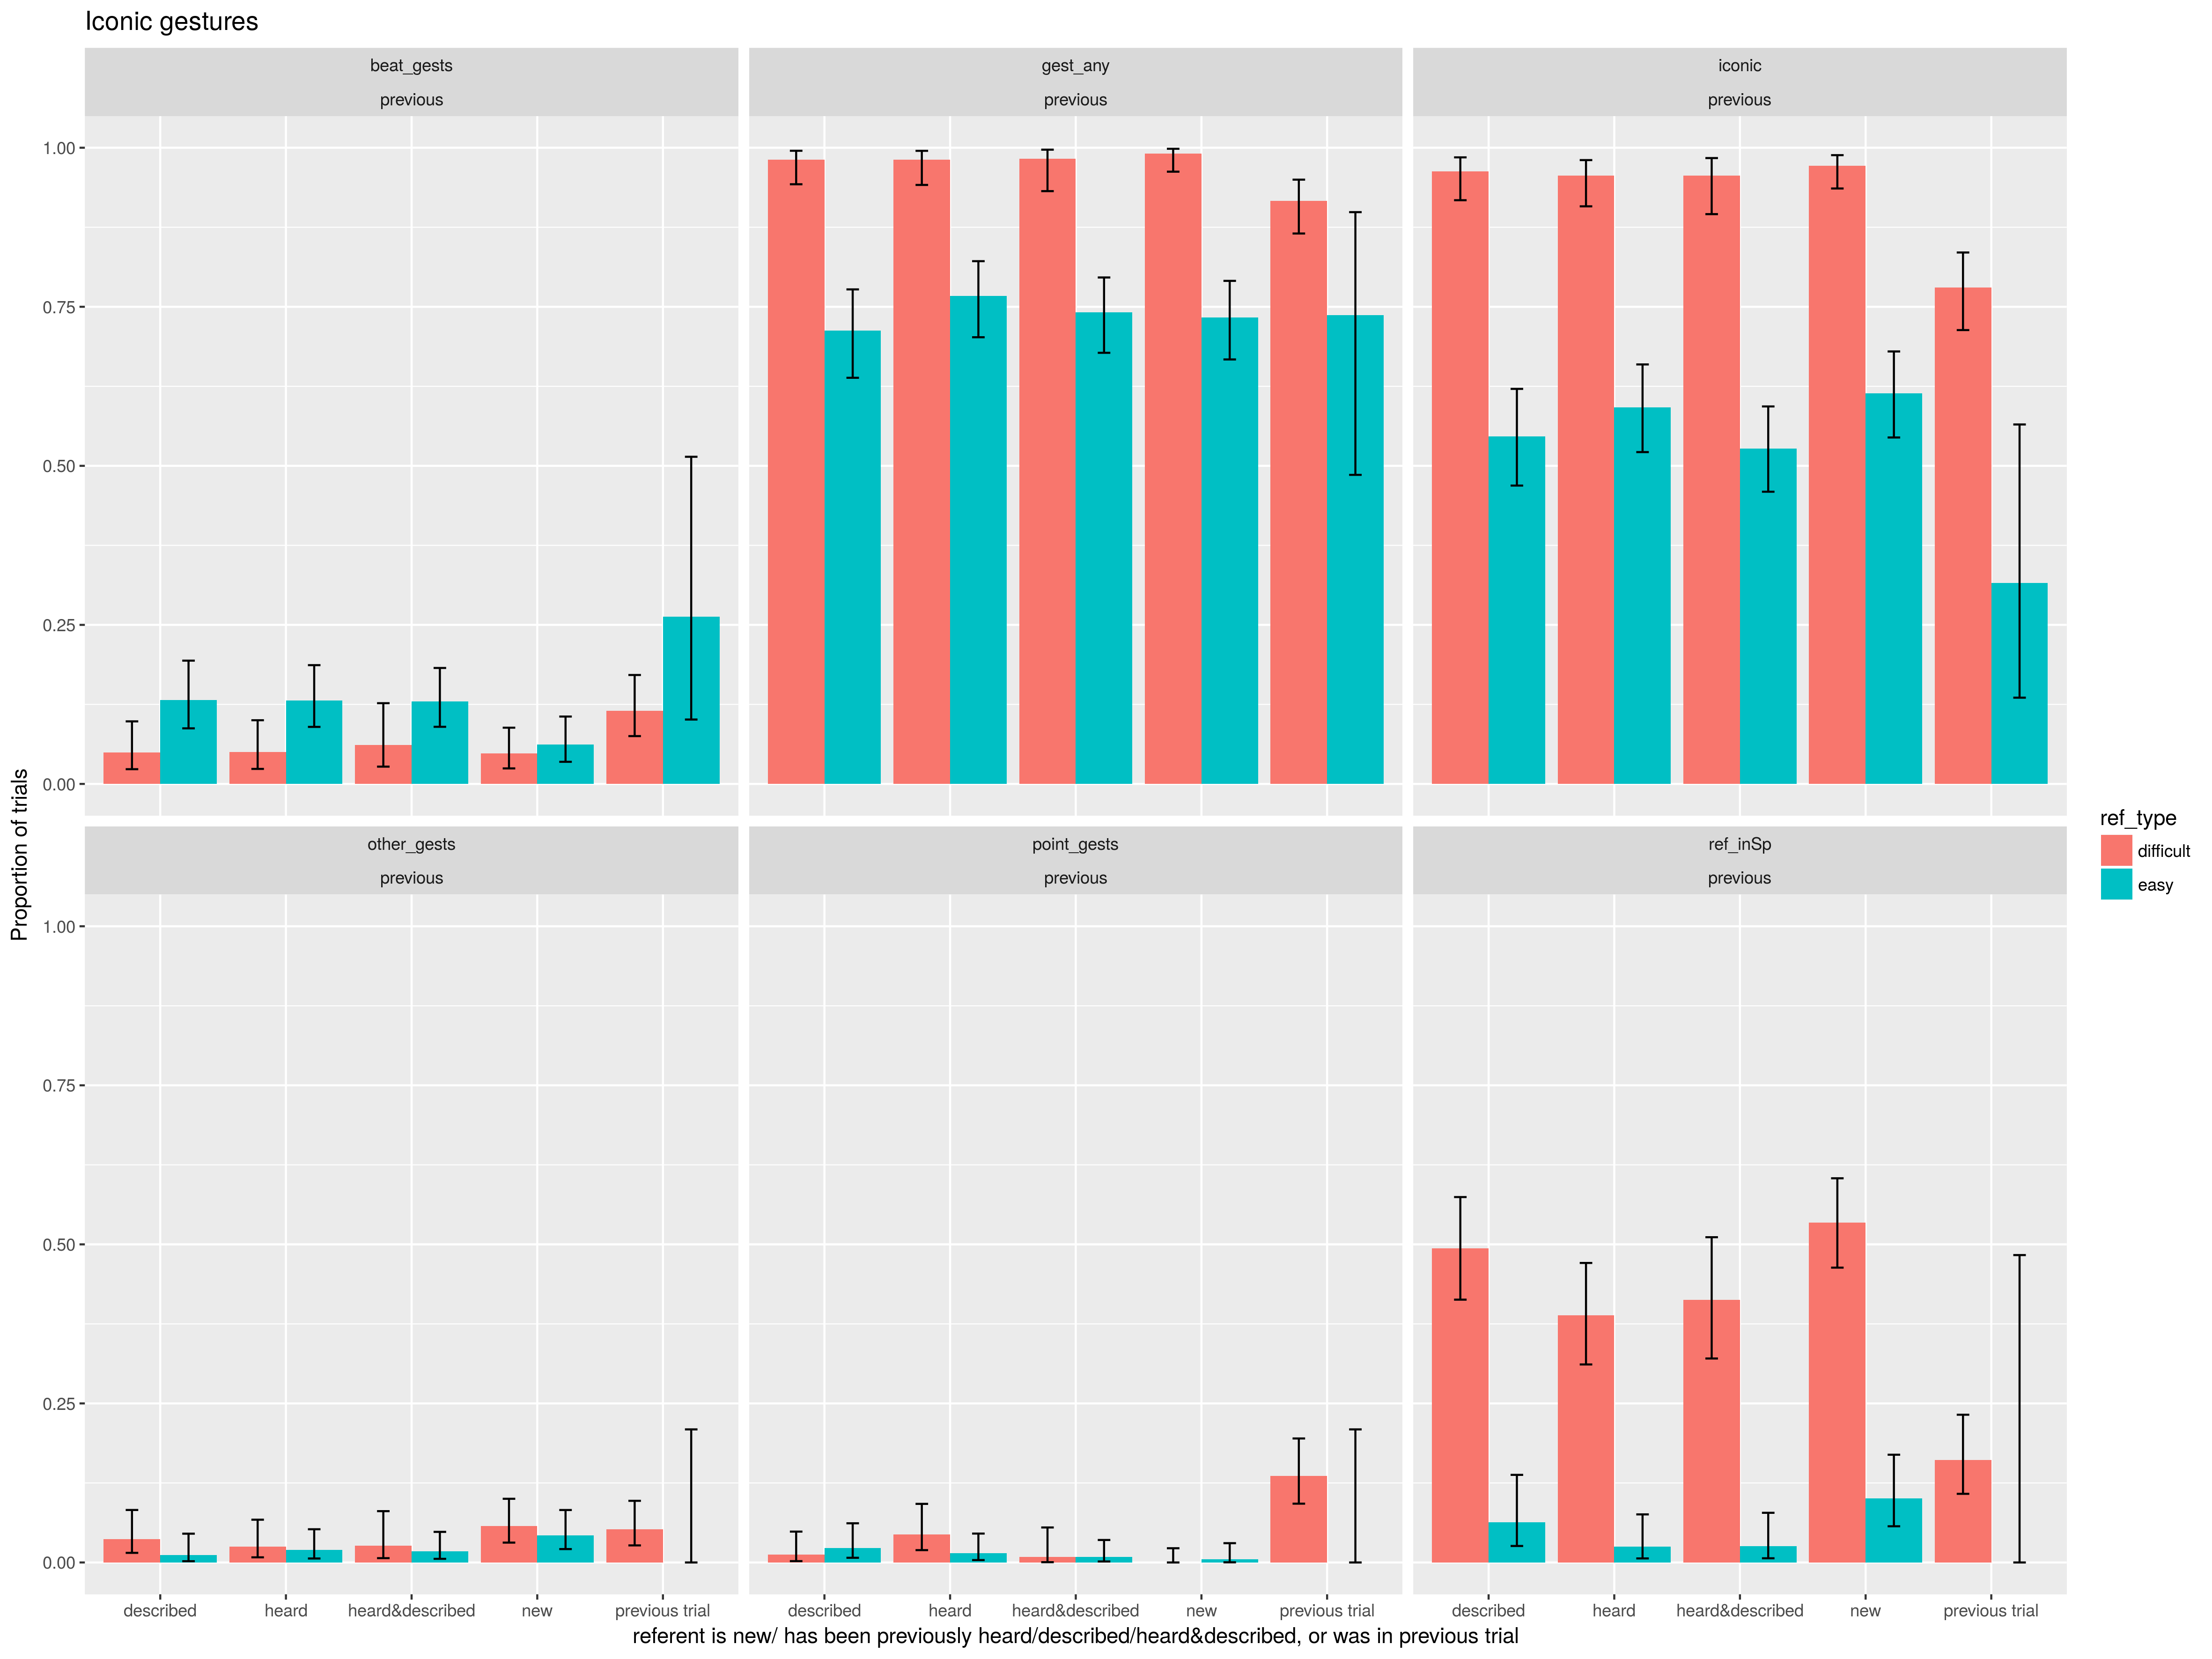
\includegraphics[width=\linewidth]{previousplot.png}
  \caption{gestures}
  \label{fig:plot}
\end{figure}

\section{discussion}
we should do a director/matcher task with varying noise. i.e. for n trials, white noise happens, making it harder to convey information via speech.
and for n trials, they have to hold something in their hands (making gesturing harder).





\bibliography{e5}

\end{document}
%%% Local Variables:
%%% mode: latex
%%% TeX-master: t
%%% End:
